\chapter{User Guide}

This section will, with the help of text and illustrations give a description of how to play the game. 

\clearpage

\section*{Game Elements}
	Here is a short description of the elements in the game. The numbers are referencing the elements in
	Figure \ref{ref:gameelements}.

	{\bf \#1: Power plant:} The power plant is able to serve buildings with power.
	A power plant has a limited amount of power and can be upgraded
	in order to serve more buildings with power. Building a power plant cost money.
	To serve buildings with power, the player must connect a power plant to
	buildings using power lines. \\
	
	{\bf \#2: Power lines: } In order to serve buildings with power, the building needs 
	to be connected to a power plant using power lines, either directly or indirectly 
	through other buildings.

	
	{\bf \#3-\#7: Buildings: } Buildings that need to be served with power will appear 
	around the map at random intervals. There are different kinds of buildings, and each 
	kind requires a different amount of power. The first building (\#1) requires the least 
	amount of power, while the last building (\#7) will require the most amount power. \\
	
	{\bf \#8: Power line status:} The power lines can have 3 different kinds of statuses.
	If a power line is connected between two building without any connection
	to a power plant, the line will be black and signalize that no power is served
	to the buildings. The same applies for power lines connecting a building to a power 
	plant that is not able to serve that building, because the other buildings connected 
	demands all its available power. The yellow line signalize that the buildings are served 
	with power. If the power line is red, it signalize that the power 
	line is damaged or unstable, and needs to be fixed. \\ 
	
	{\bf \#9: Coin:} A coin will, at regular intervals, appear next to buildings connected to
	a power plant that can serve the building with power. The coin signalize that the building 
	is receiving power form the power plant, and the owners are ready to pay for the power. The player
	can tap the coin and collect the money in order to try to reach the level specific goal of earning 
	enough money to reach the next level.

	{\bf Health bar:} If a building is not connected to a power plant, or the power line connecting 
	it to a power plant is either black or red, the building is not receiving any power and the owners 
	will leave, making the player's health bar decrease. If the health bar reaches the bottom the game is over.

	\begin{figure}[H]
		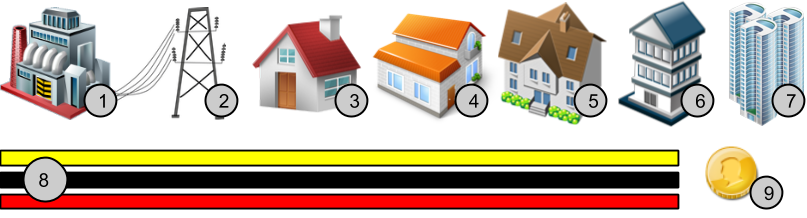
\includegraphics[width=\textwidth]{pictures/GameElements.png}
		\caption{Game elements}
		\label{ref:gameelements}
	\end{figure}

\subsection*{Map Menu}
	When a new game is started, there is a menu at the bottom of the map. The numbers are referencing 
	the elements in Figure \label{fig:mapmenuelements}. The elements in the menu are as follows:

	{\bf \#1 Money:} this is the amount of money the player has. \\
	{\bf \#2 Goal: } this is the amount of money the player needs to collect in 
	order to reach the next level.\\
	{\bf \#3 Health bar: } is the health the player has. If it reaches zero, the game is over. \\
	{\bf \#4 Build power plant: } is the element to choose if the player wants to build a power plant. \\
	{\bf \#5 Build power line: } is the element to choose if the player wants to build a power line. \\
	{\bf \#6 Pause game: } the player can tap this button to pause the game. \\

	\begin{figure}[H]
		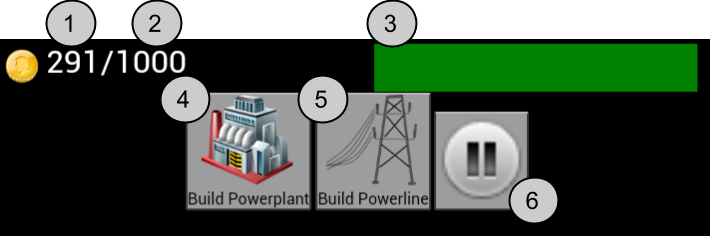
\includegraphics[width=\textwidth]{pictures/mapmenu.png}
		\caption{The map menu}
		\label{fig:mapmenuelements}
	\end{figure}

\subsection*{Start Game}

	The game always start at level 1, and the player can only reach higher levels by completing 
	all previous levels. From the main menu, the player can start a new game, see all highscores 
	or read the game instructions. 

	When the player starts a new game, an empty map will appear. The player will then be 
	presented with the goal of the level, and subsequently buildings will start appearing 
	at random positions on the map.

	The player needs to build power plants, power lines and collect money in order
	to reach the next level.

\subsection*{Build Power Plant}

	To build power plants the player taps the power plant icon at the bottom of the screen. 
	This will make the player enter building mode, and the player can tap the location on the 
	map he wants to place the power plant. 

	In order to build a power plant, the player must have enough money and the
	location that is chosen has to be empty.

\subsection*{Build Power Line}

	To build power lines the player taps the power line icon at the bottom of the screen. 
	This will make the player enter building mode and, and the player can tap the two 
	building he wants to connect with a power line. The player need to be able to afford 
	the power line to build it and the cost of the power line is proportional to the length 
	between the two buildings.

\subsection*{Repair or remove damaged Power Line}

	If a power line is damaged, it will turn red. The player needs to press on the
	damaged power line in order to fix it or remove it. 

\subsection*{Upgrade Power Plant}

	A power plant can only serve a fixed amount of power. If the player wants a power
	plant to serve more power, the player can for a certain amount of money upgrade the power 
	plant, by tapping it, and pressing upgrade. A power plant can only be upgraded up to level 5.

\subsection*{Navigate around the map}
	
	The map in the game is quite big and the player needs to navigate around
	the map in order to get an overview of all the elements on the map. 
	In order to navigate, the player swipe the finger over the screen and the 
	map position will change. In order to get a full overview of the map, the player
	only needs to double-tap the map. The map will then zoom out and the player
	can double-tap again to go back to normal map view. The player can not build in 
	the zoomed out view.

\subsection*{Pause the game}

	If the player wants to pause the game, he can press the pause button in 
	the menu or just exit the game. 

\subsection*{Collect money}
	
	When buildings are connected to a power plant, the player will be able to collect
	money from the buildings. The player is able to collect the money by pressing on the
	building with a attached coin and the players amount of money will increase. If
	the amount of money is equal or greater than the goal, the player reaches the next level.

\subsection*{Building is not served with power}

	When a building appears on the map, a countdown starts. The player needs to connect
	the building to a power plant before the countdown is zero. If the countdown is zero, 
	the building will disappear and the health bar will decrease.

\subsection*{Next level}

	The higher the level is the more difficult it will be. The rate at which buildings appear 
	will increase, the rate at which power lines are damaged will increase, and the map size increases.

\subsection*{Highscore}

	At the start of a new level, a timer will start. The player should try to complete the level as 
	fast as possible. The highscore shows the best time the player has gained at each level he has completed.